%*****************************************
\chapter{Related Work}\label{ch:related_work}
%*****************************************
%\setcounter{figure}{10}
% \NoCaseChange{Homo Sapiens}

\section{Services inside the Smart Home: A Simulation and Visualization tool}\label{sec:services_in_smart_homes}

In this work \cite{lazovik2009services} the aim is to reduce the testing costs of smart homes. The goal was achieved by implementing a simulation and visualization tool which replaces services in a smart home with virtual stubs behaving just like the real hardware installed in a house.\\

For the implementation of virtual stubs they have employed the service-oriented computing paradigm, which is widely used to implement systems requiring high interoperability, scalability, security and reliability. One of the main advantages is that such software can seamlessly integrate other systems written in other programming languages and even deployed under different operating systems.\\

The simulation scenarios are built using Google SketchUp\footnote{http://www.sketchup.com}. This was extended with a set of tools extending its visual representation of a house with virtual home interactive web services supporting SOAP messages. Further, the visualization component is written as a set of plug-ins for Google SketchUp.\\

The simulation and visualization tool allows to simulate any possible home automation scenario, with the possibility of modeling the user and its interactions with the home.

\section{Simulation of Smart Environments}\label{sec:sim_of_smart_envs}

In this work \cite{armac2007simulation}, Armac and Retkowitz introduce a tool called \emph{eHomeSimulator}, which was build in order to support the simulation of smart environments, or as the authors refer to them in the present work \emph{eHomes}. The motivation behind the work is that smart environments constitute already an important research area, but building a real eHome is associated with high effort and financial costs. Therefore, the eHomeSimulator helps in abstracting out from creating buildings (the actual physical environment) and purchasing devices, allowing us to focus only on software engineering aspects and challenges involved in eHome development (e.g. developing services, deployment etc.).\\

Describing in details the eHome is out of scope, but for clarity, we will a offer a short description. Therefore, eHome is basically a framework consisting of a hardware platform (the residential gateway) and a software platform (service gateway, runs on top of the hardware platform). The devices and appliances, which make up the eHome, are connected to the hardware platform. They are of two basic types: sensors and actuators. Sensors offer contextual information like temperature, humidity etc. while actuators can change the environment's state (e.g. a speaker, a heater etc.). The hardware platform is governed by the software platform which acts as a runtime environment for eHome services. These services can be of two types: basic and integrating. Basic service are meant to control devices (e.g. a lamp driver) while the integrating services are composed of various basic service. These services are developed based on the OSGi component model \cite{allianceosgi}, imposing a highly decoupled architecture to the service model and offering high reusability of the developed services. One novelty introduced by the architecture of the framework is that service can work both with real device and simulate device.\\

The eHomeSimulator is built on top of eHome framework to allow intuitive interaction and to visually represent the state of the simulated environment. In the evaluation process of the simulator, eHome environments consist of three main elements: rooms devices and persons (agents interacting with the environment). The graphical representation is a 2D view with a view point from top, which is built up from three layers:
\begin{itemize}
	\item The bottom layer contains the graphics to represent the background (floor, walls and furniture) build up from tiles placed one next to each other.
	\item On top of the background, there is the middle layer representing the graphics of the devices. These are only static devices and they can have different colors based on their state.
	\item The top layer represents the agents interacting with the environment. They can move freely in all accessible areas, interacting with the devices.
\end{itemize}

There is a environment editor which assists in setting up a simulated environment. The process starts by designing the room, walls and furniture using Google Sketchup \footnote{\url{http://sketchup.google.com/}} which then is uploaded into the editor. On top of this base we can further place the devices and appliances.\\

The eHomeSimulator's architecture is based on the Model View Controller design pattern \cite{erich1995design}. The model of the system holds the data structures representing the current state of the system, the view implements the graphical representation based on the current model and the controller process the user interaction with the simulator, updating the view according to changes in the model.\\

The image depicted in Figure \ref{fig:simulated_env} displays a simulation in progress. On the right side, we can observe the agent interacting with the environment while on the left side there is a control panel displaying various context data of the current status of the system and allows to interact with nearby devices (e.g. turn on/off a lamp).

\begin{figure}[H]
	\centering
	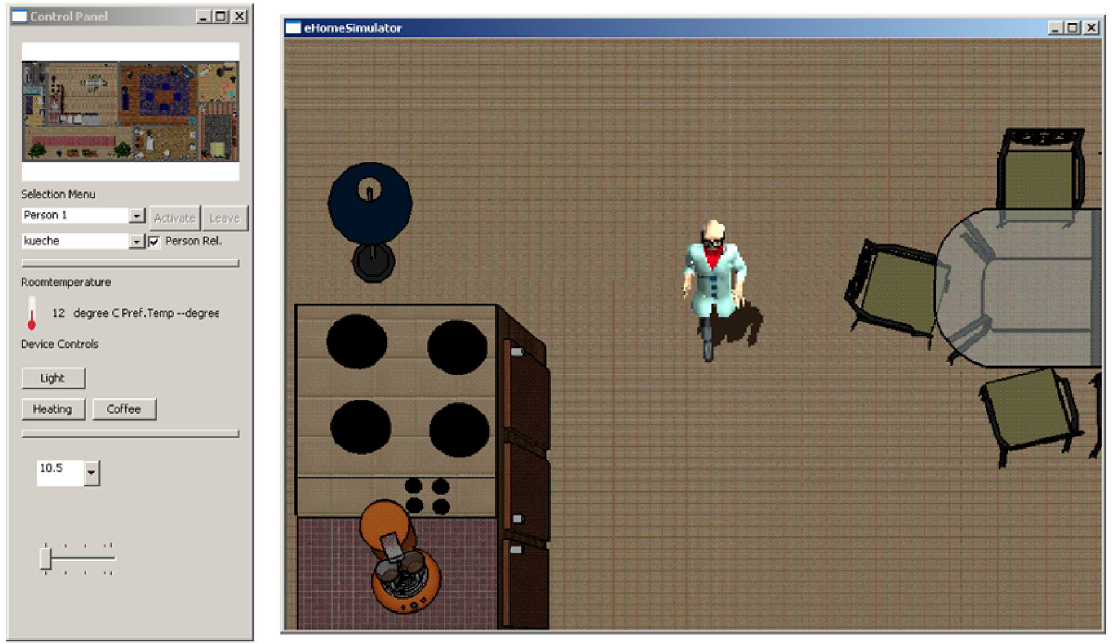
\includegraphics[width=\linewidth]{gfx/Chapter2/simulated_env}
	\caption{The GUI of the simulator}
\label{fig:simulated_env}
\end{figure}

The eHomeSimulator has an architecture providing loose coupling between components. Also, the underlying framework's architecture offers great support for reusability of services and integration with real-life devices. The devices are trivial, offering basic interactions (e.g. on/off) and they are static (the agent can't move them). Actually, all the agent can do is move around between some given bounds and interact with some of the device. There is no support for mobility of devices and wearable device, nor is it in plan for future work. Moreover, the representation of the agent is in 2D where he can be facing 4 directions, offering no support for various states like sitting, standing etc.\\

The project is close sourced, making it impossible to extend, to reuse or to contribute to it. In conclusion, there are a few lessons to be learnt from the architectural choices made within this project.

